\chapter{De lo simple a lo complejo}

Dentro del marco de los sistemas complejos se manejan varias ramas muy interesantes que le dan su esencia, desde los sistemas dinámicos discretos, dinámica no lineal, teoría de redes complejas, termodinámica fuera de equilibrio, modelos basados en agentes, entre otras. Cada una de ellas aporta un valioso contenido al sistema complejo que se quiera estudiar y analizar dependiendo de sus componentes. Delimitar el área de los sistemas complejos aún resulta una labor complicada debido a su gran \textit{diversidad}, sin embargo, se sabe de la existencia de ciertas características que todo sistema complejo comparte. Los sistemas complejos cuentan con entes: \textit{conectados, interdependientes, dependientes del camino, emergentes} entre otros. El presente trabajo tiene como propósito mostrar al lector cada una de estas características con el objeto de estudio que se va a proponer como piedra angular.\\
\\
Para llegar a conocer nuestra piedra angular primero será necesario delimitar las áreas que intervendrán en la discusión constante de este texto. Se ocupará un \textit{sistema dinámico no-lineal} bajo el soporte de una \textit{red compleja}. La Dinámica no lineal es la rama de los sistemas dinámicos continuos en donde el comportamiento del sistema no se rige por la suma de los comportamientos de sus descriptores. Por ejemplo, una neurona y la suma del comportamiento de las neuronas de un cerebro no puede explicar la emergencia de la consciencia. Por otro lado las redes complejas es la extensión de la \textit{teoría de grafos} aplicada a escenarios comunes de la naturaleza y de la vida cotidiana, tales como redes ecológicas, redes sociales, redes comerciales etc. Su importancia radica en las propiedades que se le pueden extraer para interpretar información sobre la estructura de la red y de la red misma.

\section{Revisión de sistemas lineales.}

En los cursos de ecuaciones diferenciales de cuarto semestre\footnote{citar a Blanchard y Devaney} es obligado abordar el tema de los sistemas de ecuaciones diferenciales lineales con el objetivo de explorar en un primer nivel el comportamiento de diversas cantidades que interactúan y evolucionan en el tiempo. Las ecuaciones diferenciales son la herramienta para modelar fenómenos y su evolución en el tiempo; nos permite trazar soluciones que describen su trayectoria. Dicho de otra forma, son la herramienta para anticipar el comportamiento del fenómeno aunque en la vida real no es tan simple como suena.
\begin{definición}
	Un sistema de ecuaciones diferenciales lineales es una colección de $n$ ecuaciones diferenciales interrelacionadas de la forma
	\begin{equation}\label{eqn:sistemaLineal}
		\begin{split}
			\dot{x}_1 &= f_1(x_1(t),...,x_n(t))\\
			\dot{x}_2 &= f_2(x_1(t),...,x_n(t))\\
			\vdots\\
			\dot{x}_n &= f_n(x_1(t),...,x_n(t))
		\end{split}
	\end{equation}
	donde $f:\mathbb{R}^n\to\mathbb{R}$ lineal, continua y diferenciable. No esta demás recordar que para que una función se considerada lineal debe de cumplir para cualesquiera dos vectores $u,v \in\mathbb{R}^n$ y para todo $k\in\mathbb{R}$ satisface:
	\begin{itemize}
		\item [1.] $f(u+v)=f(u)+f(v)$
		\item [2.] $f(ku)=kf(u)$
	\end{itemize}
	A este cumplimiento se le conoce como \textit{principio de superposición} y el concepto se extiende cuando contamos con las soluciones del sistema lineal.
\end{definición}
Al tratarse de un sistema lineal, resulta bastante oportuno expresarlo en términos de notación matricial, es decir, una multiplicación de una matriz cuadrada $M\in\mathcal{M}_n(\mathbb{R})$ por un vector columna que tiene a todas las funciones $x_i(t)$ lineales.
\begin{align*}
	\begin{split}
			\dot{x}_1 &= a_{11}x_1(t)+\cdots+a_{1n}x_n(t)             \\
			\vdots &\qquad \vdots\qquad\qquad\vdots\qquad\quad\vdots  \\
			\dot{x}_n &= a_{n1}x_1(t)+\cdots+a_{nn}x_n(t)             
	\end{split}	          
	\qquad\ \ \, \Longleftrightarrow
	\begin{split}
		\underbrace{\begin{pmatrix}
				\dot{x}_1\\
				\vdots\\
				\dot{x}_n
		\end{pmatrix}}_{\dot{X}(t)}=\underbrace{\begin{pmatrix}
				a_{11} & \cdots & a_{1n}\\
				\vdots & \ddots & \vdots\\
				a_{n1} & \cdots & a_{nn}
		\end{pmatrix}}_{M}\underbrace{\begin{pmatrix}
		x_1(t)\\
		\vdots\\
		x_n(t)
	\end{pmatrix}}_{X(t)}
	\end{split} 
\end{align*}
en este caso las constantes de la matriz $a_{ij}\in M$ son parámetros que describen ciertas interacciones con respecto de las cantidades que intervienen en el sistema (\ref{eqn:sistemaLineal}); estas interacciones son las responsables de la dinámica del sistema, es decir, de la manera en que evoluciona en el tiempo dependiendo de sus condiciones iniciales. Es conveniente poder contar con la matriz de coeficientes ya que por si sola nos servirá para darle solución al sistema lineal y para poder conocer la estabilidad del mismo, aún sin saber la solución general. Para ahondar en el tema de la estabilidad es necesario conocer los \textit{puntos fijos} del sistema.


%%%%%%%%%%%%%%%%%%CHECHPOINT


\subsection{Puntos fijos y estabilidad del sistema.}

También llamados puntos de equilibrio son aquellos en donde las soluciones de (\ref{eqn:sistemaLineal}) permanecen constantes en el tiempo y dependiendo de su naturaleza\footnote{dictada por los elementos de la matriz de coeficientes $M$.} se establecerá si el punto y el sistema en cuestión es estable o inestable. Para poder hallarlos es necesario hacer cumplir el siguiente sistema de ecuaciones
\begin{equation*}
	\begin{split}
		\dot{x}_1 &= f_1(x_1(t),...,x_n(t))=0\\
		\dot{x}_2 &= f_2(x_1(t),...,x_n(t))=0\\
		\vdots\\
		\dot{x}_n &= f_n(x_1(t),...,x_n(t))=0
	\end{split}
	\quad\Longleftrightarrow\quad
	\begin{split}
		\begin{pmatrix}
			a_{11} & \cdots & a_{1n}\\
			\vdots & \ddots & \vdots\\
			a_{n1} & \cdots & a_{nn}
		\end{pmatrix}
		\underbrace{\begin{pmatrix}
				x_1(t)\\
				\vdots\\
				x_n(t)
		\end{pmatrix}}_{X_0}=0
	\end{split}
\end{equation*}
Para darle solución es necesario encontrar $X_0\in\mathbb{R}^n$ que lo satisfaga; en dicho caso se establece que $X_0$ es el punto fijo del sistema. Los puntos fijos son clave para entender la estabilidad de (\ref{eqn:sistemaLineal}), servirán de referencia para determinar si las soluciones tienden hacia el punto fijo o si divergen del mismo (o una combinación de ambas). Pero tan solo con determinarlo no es suficiente, para ello debemos manipular la matriz de coeficientes $M$ para saber que tipo de punto fijo es. Para ello necesitamos hallar los \textit{valores propios} de $M$, por tanto se necesita resolver
\begin{equation}\label{eqn:vPropios}
	\det(M-\lambda I)=0
\end{equation}
al encontrar las raíces del polinomio característico de grado $n$ (dependiendo del tamaño del sistema), se obtendrá el conjunto de valores propios que por si mismos nos brindan demasiada información acerca de como se comportan las soluciones del sistema.

%%%%%%%%%%%%%%%%%%CHECKPOINT
\begin{proposición}\label{prp:Atractores}
	Un sistema lineal que tiene eigenvalores con parte real negativa siempre será estable, es decir, todas las soluciones tenderán hacia el punto fijo del sistema. Este punto de equilibrio del sistema con estas características es conocido como \textbf{Atractor}.
\end{proposición}
Independientemente de la elección de las condiciones iniciales, las soluciones tenderán hacia el punto fijo cuando $t\to\infty$ y se mantendrá ahí siendo resistente ante perturbaciones. Notemos que en la ec. (\ref{eqn:vPropios}) es posible tener raíces reales como complejas, dependiendo de los coeficientes de $M$. Sin embargo aunque se tengan eigenvalores complejos, la dinámica seguirá siendo la misma: se tendrán soluciones que tienden o divergen (o combinación de ambas) del punto fijo, lo que cambia es la forma en que lo hacen. Cuando las soluciones del sistema lineal divergen del punto fijo, entonces se establece que el sistema es inestable y el punto fijo asociado se le conoce como \textbf{\textit{Repulsor}}. Cualquier mínima perturbación que tenga la solución que esta ubicada en el punto fijo, hará que diverga. La combinación de los anteriores se les conoce como \textbf{\textit{Punto silla}}; se dice que es combinación porque podría acercarse al punto silla pero al hacerlo en algún momento terminará divergiendo. Es considerado también como sistema intestable ya que para $t\to\infty$ cualquier solución no trivial se irá a $\infty$.
\begin{ejemplo}\label{eg:Fuente2x2}
	Veamos un ejemplo sencillo para poder apreciar lo anterior, para ello se propone el siguiente sistema de $2\times 2$.
	$$
		\dot{X}(t)=\underbrace{\begin{pmatrix}
				2 & 2\\
				1 & 3
		\end{pmatrix}}_{M_1}X(t)
	$$
	Sacando su polinomio característico (\ref{eqn:vPropios}) tenemos los siguiente eigenvalores\footnote{para sistemas de $2\times 2$ se tiene establecido un polinomio característico que se define como $p_M(\lambda)=\lambda^2-\lambda\text{Tr}A+\det A$}
	\begin{align*}
		p_{M_1}(\lambda)&=\lambda^2-5\lambda+4 = 0\\
		\lambda_1=4 &\qquad \lambda_2=1
	\end{align*}
	Según lo que establece la Proposición \ref{prp:Atractores}, este no es un sistema que sea estable ya que sus eigenvalores tienen parte real positiva. Para poder comprobarlo necesitamos determinar la solución general del sistema asociado a $M_1$. Para ello es necesario encontrar los \textit{eigenvectores} del sistema, es decir
	\begin{align*}
		M_1\vec{v}=\lambda\vec{v}\qquad&\Longleftrightarrow\qquad (M_1-\lambda I)\vec{v}=0 \\
		\vec{v}_{\lambda_1} = \begin{bmatrix}
			1\\
			1
		\end{bmatrix}  \qquad&\qquad \vec{v}_{\lambda_2} = \begin{bmatrix}
		\frac{1}{2}\\
		-1
		\end{bmatrix}
	\end{align*}
\end{ejemplo}
\begin{teorema}\label{teo:Solgral}
	Sea $\vec{v}_0$ un eigenvector de $M$ una matriz asociada a un sistema de ecuaciones diferenciales lineales con $n$ eigenvalores $\Lambda=\{\lambda_i\, |\, i\in\{1,...,n\}\}$. Entonces la función $X(t)=e^{\lambda t}\vec{v}_0$ es una solución del sistema $\vec{X}(t)=MX(t)$\footnote{ver demostración en el apéndice \ref{ch:Ap}}.
\end{teorema}
Se dice que es una solución general porque podemos seleccionar cualquier $k\in\mathbb{R}$ de tal manera que sea un múltiplo del eigenvector asociado a $\lambda_i$. En ese caso obtenemos toda una familia de soluciones posibles. Por tanto para el sistema del Ejemplo \ref{eg:Fuente2x2} se tienen las siguientes soluciones
$$X_1(t)=k_1e^{4t}\begin{bmatrix}
	1\\
	1
\end{bmatrix},\qquad\qquad X_2(t)=k_2e^{t}\begin{bmatrix}
\frac{1}{2}\\
-1
\end{bmatrix}$$
Por tratarse de un sistema lineal, se cumple el principio de superposición lo cual significa que la solución general al sistema asociado a $M_1$ es
$$X(t)=k_1e^{4t}\vec{v}_{\lambda_1}+k_2e^{t}\vec{v}_{\lambda_2}$$
Se puede apreciar que para cualquiera de las soluciones del sistema asociado a $M_1$, el límite de $X(t)$ cuando $t\to\infty$ es infinito, por tanto las soluciones del Ejemplo \ref{eg:Fuente2x2} siempre van a diverger a infinito independientemente de la elección de condiciones iniciales. Cuando se trata de sistemas lineales, una solución y la suma de las soluciones siempre será solución del sistema, es decir, se pueden escribir como combinación lineal. Generalizando el concepto a un sistema de $n$ ecuaciones lineales tenemos la siguiente solución general:
\begin{equation}\label{eqn:solGral}
	X(t)=k_1e^{\lambda_1 t}\vec{v}_{\lambda_1}+k_2e^{\lambda_2 t}\vec{v}_{\lambda_2}+\cdots+k_ne^{\lambda_n t}\vec{v}_{\lambda_n}
\end{equation}
Esta solución general también aplica perfectamente para el caso en donde se tienen eigenvalores complejos, solamente habría que descomponer las exponenciales con base en la relación de Euler, es decir, $e^{\lambda t}$ donde $\lambda=a\pm bi$ se descompone como $e^{at}\left (\cos bt+i\sin bt\right )$. Como solución se vería de la siguiente manera
\begin{equation}\label{eqn:solCompleja}
	X(t)=e^{at}\left (\cos bt+i\sin bt\right )\vec{v}_{\lambda}
\end{equation}
la forma en que se comportarán las soluciones ya sea que convergan o divergan del punto fijo es mediante oscilaciones que crecen o decrecen en función de $e^{at}$. Llegando a este punto tenemos todos los elementos para darle soporte a nuestra Proposición \ref{prp:Atractores}; tanto la ecuación (\ref{eqn:solGral}) como (\ref{eqn:solCompleja}) se puede notar que si la parte real del eigenvalor del sistema es positivo, para $t\to\infty$ la exponencial también tiende a infinito y por lo tanto la solución lo hará. En contra parte, si la parte real del eigenvalor es negativa entonces la solución va a tender hacia donde los vectores propios se dirijan, particularmente hacia el punto fijo. Esto únicamente será válido si todos los eigenvalores del sistema tienen parte real negativa ya que si existe al menos uno que tenga parte real positiva eventualmente terminará divergiendo. Es lo que sucede con los puntos silla, quizás existan mayoría de eigenvalores con parte real negativa pero si existe al menos uno que tenga parte real positiva, eventualmente para tiempos largos la solución va a diverger. Para poder darnos una idea visual de lo que llamamos \textit{atractores}, \textit{repulsores} y \textit{puntos silla} podemos acceder al espacio fase del sistema y ver de manera integral como se comportan las soluciones del sistema lineal.
%%%%%%%%%%%%%%%%%%%%%%%%%CHECKPOINT
\subsection{Espacios fase}\label{sec:Espacios fase}

El espacio fase es considerado como la representación geométrica de las trayectorias posibles en un sistema dinámico, en el mismo se contemplan todas las condiciones iniciales posibles y todas las trayectorias posibles que emergen de las anteriores. Aquí mismo encontramos gráficamente los puntos fijos y podemos distinguirlos cualitativamente de que naturaleza son. Las técnicas analíticas descritas anteriormente nos sirven para conocer el comportamiento sin el uso del espacio fase, pero para sistemas de $n=2,3$ podemos acceder al espacio fase y ver como son sus trayectorias. En ese sentido para sistemas con $n>3$ ecuaciones ya será imposible generar su visualización ya que cada uno de los ejes representa una de las cantidades del sistema. \\
\\
En esta breve sección únicamente veremos diversos ejemplos de sistemas $2\times 2$ con eigenvalores variados que nos muestren atractores, repulsores y puntos silla. Sin embargo se omitirán los cálculos de eigenvalores, eigenvectores y soluciones generales, únicamente se pretende mostrar al lector como podemos analizar los sistemas de manera cualitativa a través de sus espacios fase. Por último se dividirán entre espacios fase con eigenvalores reales y con eigenvalores complejos para tener una demarcación adecuada de ambos casos.
\newpage
\begin{ejemplo}\label{eg:EspaciosFreal}
	Para la sección de espacios fase con eigenvalores reales vamos a considerar las siguientes matrices de coeficientes para $n=2$
	\begin{equation*}
		\begin{split}
			R_1=\begin{pmatrix}
				-1 & 0\\
				0 & -4 
			\end{pmatrix}
		\end{split},\qquad
		\begin{split}
			R_2=\begin{pmatrix}
				-3 & 0\\
				0 & 2 			
			\end{pmatrix}
		\end{split},\qquad
		\begin{split}
			R_3=\begin{pmatrix}
					2 & 2\\
					1 & 3
			\end{pmatrix}
		\end{split}
	\end{equation*}
	Nótese que la $R_3$ es la misma que la $M_1$ del Ejemplo \ref{eg:Fuente2x2} la cual tiene ambos eigenvalores positivos y se había concluido que sus soluciones divergen del punto fijo con base en la solución general (\ref{eqn:solGral}); además en la Figura (\ref{fig:EFReales}) se puede observar la gráfica de la derecha que corresponde con $R_1$ como todas las soluciones divergen del punto fijo. Los eigenvalores de $R_1$ son respectivamente $\lambda_{1R_1}= -1$ y $\lambda_{2R_1}=-4$; ambos son negativos y cumplen con lo que estipula la Proposición \ref{prp:Atractores} y se puede comprobar por medio de la solución general o el gráfico de la izquierda de la Figura (\ref{fig:EFReales}) que las soluciones convergen al punto fijo. Para los eigenvalores de $R_2$ se tienen los siguientes eigenvalores $\lambda_{1R_2}=-3$ y $\lambda_{2R_2}=2$; en este caso se tiene que una de las soluciones de la ec. (\ref{eqn:solGral}) tratará de acercarse al punto fijo debido a la exponencial con $\lambda<0$, sin embargo para $t\to\infty$ las soluciones divergerán a $\pm\infty$; a partir del gráfico de en medio de la Figura (\ref{fig:EFReales}) se puede apreciar este comportamiento.
	\begin{figure}[h!]
		\centering
		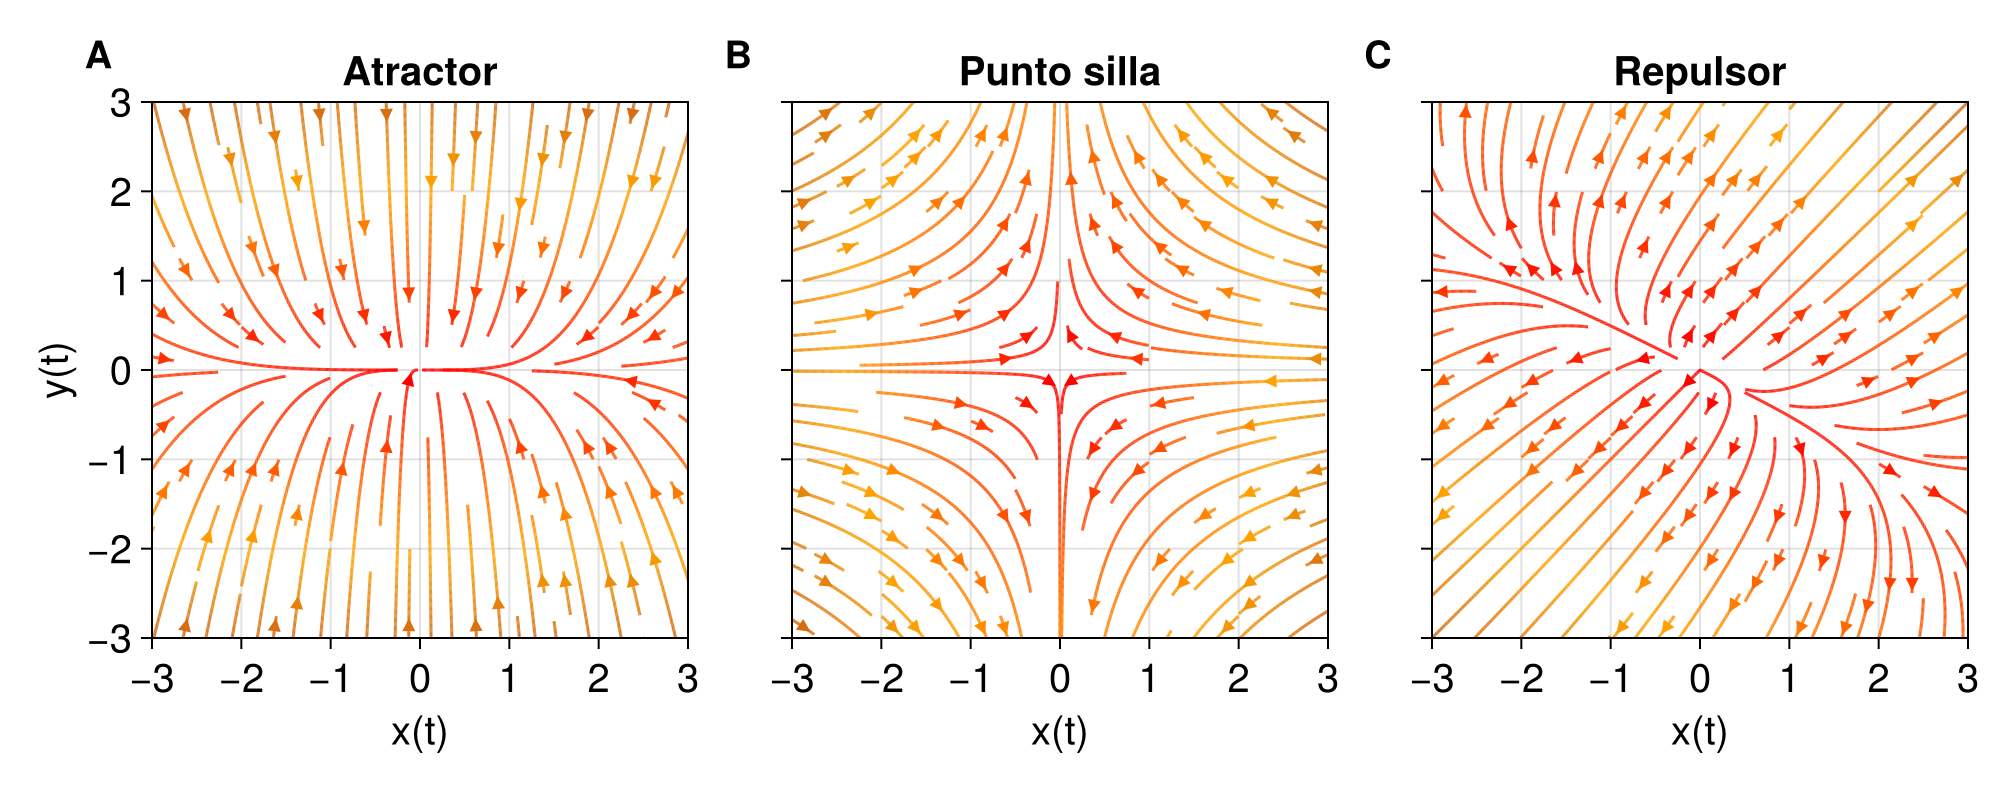
\includegraphics[scale=0.23]{../Imagenes/Espacios fase reales}
		\caption{Espacios fase con eigenvalores reales. (\textbf{A}) Corresponde con la matriz $R_1$; (\textbf{B}) corresponde con la matriz $R_2$; (\textbf{C}) corrresponde con la matriz $R_3$ del Ejemplo \ref{eg:EspaciosFreal}.}
		\label{fig:EFReales}
	\end{figure}
\end{ejemplo}

\begin{ejemplo}\label{eg:EspaciosFcomplejos}
	Para el caso de los espacios fase con eigenvalores complejos se proponen las siguientes matrices de coeficientes para $n=2$
	\begin{equation*}
		\begin{split}
			C_1=\begin{pmatrix}
				-2 & -3\\
				3 & -2 
			\end{pmatrix}
		\end{split},\qquad
		\begin{split}
			C_2=\begin{pmatrix}
				0 & 1\\
				-2 & 0 			
			\end{pmatrix}
		\end{split},\qquad
		\begin{split}
			C_3=\begin{pmatrix}
				0 & 2\\
				-3 & 2
			\end{pmatrix}
		\end{split}
	\end{equation*}
	%%%%CHECKPOINT
	Los eigenvalores para la matriz $C_1$ son $\lambda_{C_1}=-2\pm 3i$, nuevamente notamos que la parte real de sus eigenvalores son negativas lo que significa que todas las soluciones tenderán hacia el punto de equilibrio independientemente de sus condiciones iniciales; en la gráfica de la izquierda de la Figura (\ref{fig:EFComplejos}) se puede apreciar este comportamiento. Los eigenvalores de $C_2$ son respectivamente $\lambda_{C_2}=\pm 2i$, en este caso la parte real es igual a cero lo que significa que las soluciones van a estar oscilando de un determinado valor a otro sin llegar a converger a ningún punto para $t\to\infty$ . Únicamente puede cambiar la amplitud de las oscilaciones y esto dependerá de las condiciones iniciales que se impongan. Este es el comportamiento descrito por el \textit{oscilador armónico simple} y sabemos que es considerado como ideal ya que en la naturaleza no se conocen cantidades que oscilen de manera perpetua y sin pérdida de energía. Por último los eigenvalores de $C_3$ son respectivamente $\lambda_{C_3}=1\pm 5i$, en este caso las soluciones divergen como se puede apreciar en la gráfica de la derecha de la Figura (\ref{fig:EFComplejos}). La parte real de sus eigenvalores es positiva lo que indica dicho comportamiento para cualquier condición inicial en $t\to\infty$.
	\begin{figure}[h!]
		\centering
		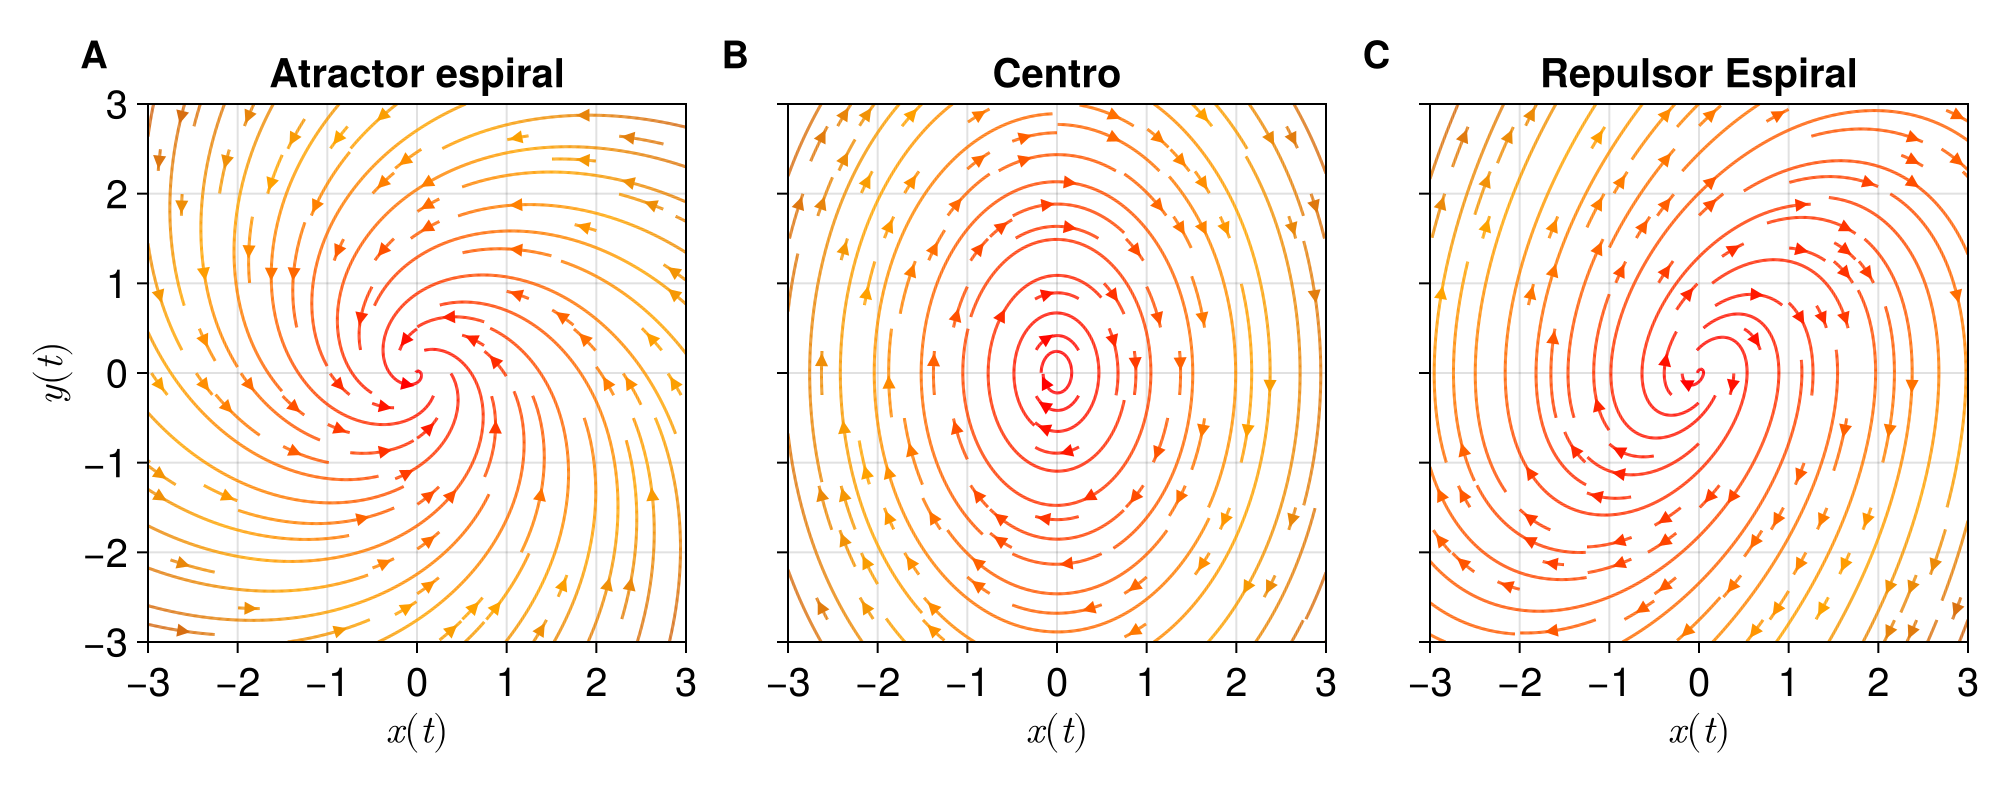
\includegraphics[scale=0.23]{../Imagenes/Espacios fase complejos}
		\caption{Espacios fase con eigenvalores complejos. (\textbf{A}) corresponde con la matriz $C_1$; (\textbf{B}) corresponde con la matriz $C_2$; (\textbf{C}) corresponde con la matriz $C_3$ del Ejemplo \ref{eg:EspaciosFcomplejos}.}
		\label{fig:EFComplejos}
	\end{figure}
\end{ejemplo}
%%%%%%%CHECPOINT
Para terminar esta sección conviene remarcar el significado de la estabilidad e inestabilidad de los sistemas y sobre todo darle una interpretación física. Ya se ha visto que cuando un sistema es estable todas sus soluciones tienden hacia el punto fijo; la estabilidad radica en que para cualquier perturbación del sistema, este siempre regresará a su punto de equilibrio y permanecerá ahí para $t\to\infty$. A diferencia de los sistemas inestables, en donde si se encuentra en el punto de equilibrio cualquier mínima perturbación hará que nunca regrese a dicho estado y cambie totalmente su dinámica. En este sentido a los primeros sistemas se les denomina como \textit{robustos} mientras que a los segundos se les denomina como \textit{sensibles}. Para la dinámica de los centros, anteriormente nos referíamos a oscilaciones perpetuas que no tienden o divergen de ningún punto de equilibrio. El sistema que representa este comportamiento por excelencia es el péndulo simple considerado como sistema ideal cuya solución se encuentra en términos de senos y cosenos. \\
\\
Para ejemplificar los puntos de equilibrio estables o intestables pensemos en un péndulo de una vara con una masa en uno de sus extremos; un punto fijo atractor es para cuando el péndulo apunta hacia abajo ya que cualquier perturbación sea pequeña o grande hará que regrese a su estado de equilibrio. En contraparte si conseguimos que el péndulo permanezca estable apuntando hacia arriba, cualquier mínima perturbación hará que nunca regrese a ese estado de equilibrio. Para este ejemplo en particular, si perturbamos el estado de equilibrio inestable terminará posicionándose en el estado de equilibrio estable para algún tiempo considerablemente.


\section{Sistemas no lineales}
%%%%%%% CHECKPOINT
El enfoque principal de este trabajo es en sistemas de ecuaciones diferenciales no lineales. No obstante, ha sido pertinente abordar el tema de los sistemas lineales para poder introducir los conceptos que serán de utilidad y que se extienden al terreno de algunos sistemas de ecuaciones diferenciales no lineales. Tal y como lo dice el nombre, un sistema no lineal es aquel en el que el conjunto de ecuaciones de (\ref{eqn:sistemaLineal}) es no lineal; significa que las ecuaciones que lo componen tienen términos no lineales tales como funciones trigonométricas, exponenciales, cuadradas, cúbicas etc. Esta característica quita la posibilidad de poder expresarlo en términos de una transformación lineal, particularmente en su forma matricial, y como consecuencia de ello: el principio de superposición ya no se cumple. Esto implica que para dados dos vectores $u,v\, \in\mathbb{R}^n$ y para todo $k\in\mathbb{R}$ se tiene lo siguiente
$$f(k(u+v))\neq k\left (f(u)+f(v)\right )$$
De misma manera, esto se extiende a las soluciones del mismo sistema: ahora la suma de sus soluciones no será solución del mismo. Como bien se mencionaba al principio del capítulo, esto tiene implicaciones interesantes ya que la suma de las componentes genera un sistema complejo que es más que la suma de sus partes tal y como lo puede ser un Huracán, una colonia de hormigas de la que emerge auto-organización etc. Queda preguntarse sobre el carácter de las soluciones; aunque el \textit{Teorema de existencia y unicidad} pueda extenderse hasta ciertas ecuaciones no lineales, éstas deben de cumplir sus hipótesis para que pueda aplicar\footnote{También conocido como Teorema de Picard-Lindelöf. Se deben cumplir las siguientes hipótesis para que se pueda aplicar el teorema: se considera $f:\Omega\subseteq (\mathbb{R}\times\mathbb{R}^n)\to\mathbb{R}^n$, donde $\Omega$ es un conjunto abierto y $f$ una función continua y localmente Lipshcitz con respecto de $x$; en caso contrario la ecuación no lineal o el conjunto de ecuaciones no lineales podrían tener soluciones múltiples. [Referenciar el teorema con demostración]}. En otras palabras, solo un determinado número de formas de ecuaciones podrán satisfacer la unicidad de la solución, el resto de casos tendrán la posibilidad de tener múltiples soluciones y más aún si se trata de un sistema de ecuaciones como el que iremos a analizar más adelante.\\
\\
En una ecuación no lineal se tiene la particularidad de que las variables dependientes y sus derivadas aparecen de forma no lineal, esto genera dependencias complejas que difícilmente se pueden simplificar lo que provoca que puedan existir las múltiples soluciones de la misma. En esta dirección, las ecuaciones no lineales producen comportamientos impredecibles al mismo tiempo que son sensibles ante condiciones iniciales lo que se resume en el amplio concepto conocido como \textit{Caos}. Normalmente de las ecuaciones no lineales emergen comportamientos caóticos aún tratándose de sistemas deterministas. Explorar las propiedades caóticas de sistemas no lineales es una propuesta interesante para investigar.\\
\\
Por lo visto, resolver ecuaciones no lineales o un sistema de ecuaciones no lineales puede ser hasta imposible si nos atrevemos a hacerlo de manera analítica. El famoso problema de los 3 cuerpos fue aquel que pudo paralizar a los científicos durante aproximadamente 200 años porque no se hallaba una solución concreta y aunque al final Henri Poincaré se le consideró como aquel que le dio respuesta\footnote{citar dicha respuesta}: dicha respuesta no fue una solución analítica que mostraba las posiciones de los planetas en función del tiempo, sino más bien concluyó que mínimas variaciones en el sistema podrían desencadenar grandes y radicales cambios a largo plazo. Con esta aseveración se establecen los pilares de la conocida \textit{Teoría del Caos} que irá floreciendo durante el siguiente siglo hasta nuestros días.\\
\\
Debido a que resulta imposible o muy complejo resolver ecuaciones no lineales de forma analítica se opta por recurrir a técnicas computacionales de integración numérica para poder obtener una aproximación de la solución del sistema no lineal y de esta manera conocer la dinámica que produce. La fidelidad de las aproximaciones numéricas depende de varios factores tales como: el método numérico empleado, el paso de integración, el tipo de ecuación o ecuaciones, condiciones iniciales etc. \\
\\
Para ecuaciones diferenciales ordinarias se tienen dos métodos principales que se enseñan en los cursos de Física Computacional e inclusive en algunos cursos de Ecuaciones Diferenciales 1: el método de \textit{Euler} y el método de \textit{Runge-Kutta} de cuarto orden\footnote{poner referencia directa del libro.}. El primero suele ser fácil de implementar debido a su simpleza, sin embargo no llega a ser muy preciso cuando se trata de ecuaciones no lineales ya que comete errores de truncamiento grandes. El método de Euler es considerado de primer orden e implica que el error local es proporcional al cuadrado del tamaño del paso de integración $O(h^2)$ mientras que para el caso de Runge-Kutta que es de cuarto orden, su error es proporcional a la quinta potencia del paso de integración $O(h^5)$, por ello es considerado uno de los métodos de integración más precisos.\\
\\%%%%%%%%CHECKPOINT
El paso de integración también toma un papel importante en la precisión de los métodos numéricos, entre más fino sea se tendrá una mejor aproximación. Debido al orden de los errores que tiene Euler y RK4 se sabe directamente que el segundo es mucho más preciso. Para el caso de sistemas no lineales es conveniente utilizar RK4 para evitar que la solución aproximada diverga de la solución real a causa de las pequeñas variaciones que se puedan producir debido al error que presenta el método. En ese sentido Euler es inestable por el orden del error que presenta, en aproximaciones numéricas a sistemas no lineales los errores se acumulan con el tiempo y llega a ser problemático ya que las variaciones que presente en las primeras iteraciones pueden ir creciendo hasta alejarse drásticamente del resultado esperado\footnote{Ver comparativa en la sección \ref{sec:SolPresaDepredador} con la Figura (\ref{fig:Rk4vsEuler}).}. RK4 es un método que se considera \textit{convergente} ya que a medida que el paso de integración $h\to 0$, la aproximación se asemeja más a la solución real y es por ello que se ha escogido este método como integrador estrella del sistema que se irá a analizar.\\
\\
A continuación se definen las reglas que deben de seguir cada uno de los métodos propuestos para generar el su respectivo algoritmo. El método de Euler sigue la siguiente correspondencia
\begin{equation}\label{eqn:Euler}
	y_{n+1}=y_n+hf(y_n,t_n)+O(h^2)
\end{equation}
Mientras que el método de Runge-Kutta de orden 4 sigue la siguiente correspondencia.
\begin{equation}\label{eqn:RK4}
	\begin{split}
		Y_1 &= y_n\\
		Y_2 &= y_n+\frac{h}{2}f(Y_1,t_n)\\
		Y_3 &= y_n+\frac{h}{2}f\left (Y_2,t_n+\frac{h}{2}\right )\\
		Y_4 &= y_n+hf\left (Y_3,t_n+\frac{h}{2}\right )\\
		y_{n+1} &= y_n+\frac{h}{6}\left [f(Y_1,t_n)+2f\left (Y_2,t_n+\frac{h}{2}\right)+ 2f\left (Y_3,t_n+\frac{h}{2}\right )+f(Y_4,t_n)\right ]+O(h^5)
	\end{split}
\end{equation}
Se pueden consultar ambos métodos y sus deducciones en las siguientes bibliografías [Poner CITAS]\footnote{poner citas}. En la sección (\ref{sec:algoritmos}) se muestra la implementación computacional de ambos métodos numéricos en el lenguaje de programación \julia.
%%%%%%%%%%%%CHECPOINT
\subsection{Modelo logístico}

En los cursos de Ecuaciones Diferenciales I se suele iniciar con la introducción del tema del crecimiento de cantidades: ya sea poblaciones, tasas de interés, etc. Para ello se presenta una primera ecuación diferencial que plantea que la velocidad de crecimiento de dicha cantidad es proporcional a su tamaño actual.
\begin{equation}\label{eqn:CrecimientoExponencial}
	\frac{dN(t)}{dt}=rN(t)
\end{equation}
en este caso a $r\in\mathbb{R}^+$ se le conoce como la \textit{tasa de crecimiento} de la cantidad. Mediante la técnica de separación de variables se deduce que la solución de esta ecuación diferencial es $N(t)=ke^{rt}$ con $k\in\mathbb{R}$. Como modelo de crecimiento poblacional es un buen punto de partida pero tiene un problema: la solución para tiempos largos diverge a $\infty$, lo que implica que la población crezca sin límites algo de lo que con certeza se sabe que es imposible. Extendiendo esta ecuación y resolviendo esta complicación se genera la propuesta del \textit{Modelo logístico}: ampliamente utilizado como base para el análisis de dinámica poblacional, propagación de enfermedades y en esencia sistemas que presenten crecimiento limitado por recursos. La ecuación logística se presenta de la siguiente forma
\begin{equation}\label{eqn:EqLogistica}
	\frac{dN}{dt}=rN\left (1-\frac{N}{K}\right )
\end{equation}
considerando que $N(t)$ es una población y $r$ es la misma tasa de crecimiento que en (\ref{eqn:CrecimientoExponencial}), $K$ se denomina como la capacidad de carga de la población. A este concepto se le entiende como el límite hasta donde puede llegar el crecimiento de esta población aún cuando la condición inicial de (\ref{eqn:EqLogistica}) se encuentre por arriba o por debajo de $K$. 
\begin{figure}[h!]
	\centering
	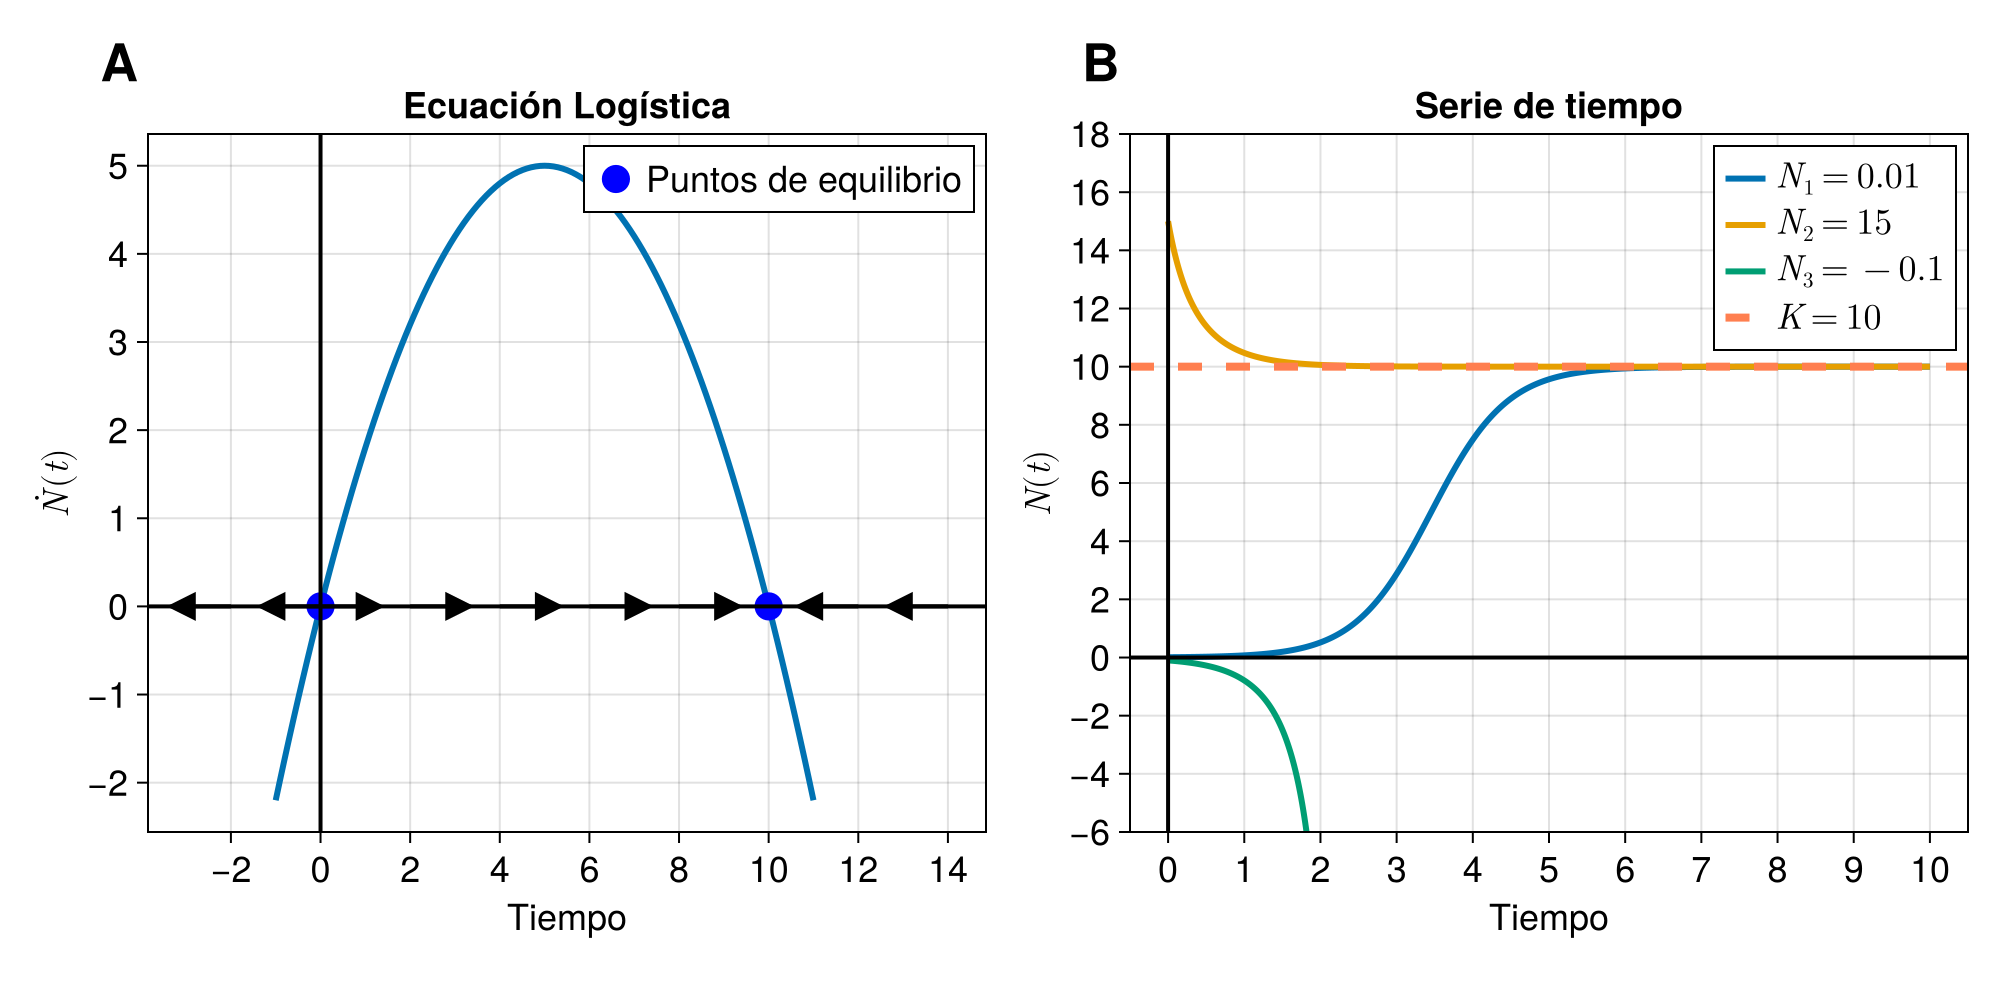
\includegraphics[scale=0.23]{../Imagenes/Ecuacion Logistica}
	\caption{Ecuación logística con una tasa de crecimiento $r=2$ y una capacidad de carga $K=10$. \textbf{A}) Se muestra su linea fase con sus puntos de equilibrio y sus respectivas estabilidades, donde el 0 es repulsor y el 10 es atractor. (\textbf{B}) Solución de la ecuación logística para las condiciones iniciales: $N_1=0.01$, $N_2=15$, y $N_3=-0.1$; se aprecia otra perspectiva de la estabilidad de los puntos fijos.}
	\label{fig:EcuacionLogistica}
\end{figure}		
La ecuación logística es no lineal ya que posee un término cuadrático pero es de las pocas a las que se le puede hallar una solución analítica\footnote{En la sección (\ref{sec:SolEqLogistica}) se muestra el proceso para hallar la solución de la ecuación logística y su comparación en series de tiempo entre la solución analítica y la solución numérica usando Runge-Kutta de orden 4.}. Consta de un crecimiento exponencial que se ve frenado por el término que se encuentra entre paréntesis. Para cierto $t^*\in\mathbb{R}^+$ se tendrá que $N(t^*)=K$ y por lo tanto la ecuación se hace cero y la población deja de crecer estableciéndose sobre la capacidad de carga: considerado como punto fijo atractor. Si se escoge una condición inicial tal que $N_0<K$ entonces la población crecerá hasta converger en la capacidad de carga,  sin embargo, si $N_0>K$ entonces la población decrecerá hasta estacionarse en la capacidad de carga (Figura \ref{fig:EcuacionLogistica}). En el caso en donde se elige una condición inicial $N_0<0$ la población simplemente diverge. Poblaciones negativas no tienen sentido de manera física por lo que las condiciones iniciales menores a cero no se toman en cuenta para la dinámica de poblaciones. \\
\\
Con base en los elementos de la sección anterior, la ecuación logística posee dos puntos de equilibrio: $\mathcal{N}=\{0,K\}$. Por tratarse de una ecuación, la dinámica se estudia en una dimensión: es decir, el espacio fase corresponde con una línea fase. Para analizar la estabilidad de los puntos fijos se suele seguir las siguientes reglas: si $\dot{N}<0$ entonces las soluciones decrecen y/o se mueven hacia la izquierda; en caso contrario $\dot{N}>0$ las soluciones se mueven y/o crecen hacia la derecha. Con base en esas reglas se puede observar la dinámica de los puntos fijos, conlcuyendo que el $0$ es un punto fijo repulsor, mientras que el $10$ es un punto fijo atractor. Físicamente tiene sentido ya que toda población en un principio comienza a crecer tendiendo hacia su punto de equilibrio estable, incluso si rebasa su capacidad de carga decrecerá hasta asentarse en su punto de equilibrio; la capacidad de carga se le interpreta en este caso como la cantidad de recursos disponibles para una población, si la población excede a la capacidad que tiene el ambiente de proveer a la población, esta va a decrecer debido a que no se cumple la demanda del tamaño de la población. En conclusión: cualquier mínima población (``perturbación") hace que la población diverga del 0 mientras que toda perturbación alrededor de $K$ hará que regrese a su estado de equilibrio.\\
\\
Se puede observar en la Figura (\ref{fig:EcuacionLogistica}: \textbf{A}) como existe un punto máximo en donde cambia la forma de crecimiento de la población, incluso en la Figura (\ref{fig:EcuacionLogistica}: \textbf{B}) se puede observar un punto de inflexión que coincide con el punto máximo de \textbf{A} y que demarca el cambio de crecimiento de la población. Ese cambio se encuentra para $N(t)=K/2$ de forma que en un principio la población crece de manera exponencial hasta que llega a $K/2$ y a partir de aquí comienza a decrecer el ritmo de crecimiento hasta llegar a su punto de equilibrio. Esta dinámica se presenta como más realista gracias a la consideración de la capacidad de carga, sin embargo aún presenta algunas limitaciones pues hay variables que existen en la realidad y que en esta ecuación no se están tomando en cuenta.\\
\\
El modelo es adecuado para tener un primer acercamiento a las dinámicas de poblaciones, sin embargo como se ha mencionado, se queda corto para ajustarse a situaciones realistas ya que no toma factores ambientales que puedan afectar a la dinámica. Por ejemplo la tasa de crecimiento únicamente depende del tamaño de la población y de no de otros factores que podrían ser más complejos tales como interacciones intraespecíficas, mortalidad, etc; la capacidad de carga también se maneja constante cuando podría ser una función del tiempo siendo afectada por elementos del entorno, tales como el clima que pueda dar lugar a sequías o abundancia de vegetación. Por lo tanto es posible acomplejar el modelo tanto como se requiera para investigar algún elemento en concreto como por ejemplo puede ser la depredación o la competencia entre diversas especies.
%%%%%%CHECHPOINT
\subsection{Modelo presa-depredador}

Uno de los sistemas no lineales más importantes aplicado a más de una especie es el modelo de presa-depredador o también conocido como Lotka-Volterra, en particular se aplica a dos especies (por lo tanto son dos ecuaciones) aunque podría extenderse a más especies. Este modelo también posee limitaciones como las que se comentaron al final de la sección anterior, sin embargo sigue siendo un modelo base para entender dinámicas de poblaciones, siendo para este caso bajo un contexto de depredación. El modelo consta de dos especies: una que es presa (la cual es consumida por la depredadora) y la depredadora (que depende de la presa para su supervivencia) y sigue las siguientes reglas\footnote{En la sección (\ref{sec:SolPresaDepredador}) se muestra la solución (implícita) del sistema presa de predador junto con la comparación de las curvas de nivel de la solución analítica contra las del espacio fase generadas por las ecuaciones de (\ref{eqn:PresaDepredador}).}
\begin{equation}\label{eqn:PresaDepredador}
	\begin{split}
		\frac{dx}{dt} &= \alpha x - \beta xy\\
		\frac{dy}{dt} &= \delta xy -\gamma y
	\end{split}
\end{equation}
En este sistema $x(t)$ corresponde con la especie de presas y $y(t)$ es la especie depredadora; $\alpha$ corresponde con la tasa de crecimiento de la especie de presas en ausencia de la especie depredadora, $\beta$ es la tasa de depredación y corresponde con la cantidad de presas cazadas, $\delta$ es la tasa de crecimiento de las presas a causa del consumo de las presas y $\gamma$ es la tasa de mortalidad de la especie depredadora en ausencia de presas. La especie presa $x(t)$ crece a diferentes ritmos en el tiempo aún con su tasa de crecimiento constante, esto debido a que se ve frenada en función de como crecen los depredadores $y(t)$ que disminuyen su población. Al mismo tiempo, los depredadores $y(t)$ irán creciendo conforme el número de presas disminuya pero en algún punto el número de presas disminuirá tanto que no satisfará la demanda de los depredadores, por lo tanto por insuficiencia los depredadores comenzarán a disminuir. \\
\\
Los ritmos de crecimiento de ambas especies vendrá dictada por los coeficientes de interacción y ciertas combinaciones entre coeficientes hace la predominancia de una de las dos especies. En concreto $\beta$ y $\gamma$ ayudan a que las presas predominen en cantidad mientras que $\alpha$ y $\delta$ hacen el mismo papel pero con los depredadores. Para el primer caso $\beta >\alpha$ y $\gamma>\delta$, esto se traduce en que existirá una alta tasa de depredación con respecto de la natalidad de las presas, significa que hay mucho consumo de presas aún cuando no nacen tantas y aunado con el hecho de que se tiene una alta tasa de mortalidad por ausencia de presas hace que disminuya drásticamente el número de depredadores. Esto permite que mientras los depredadores se ven en crisis de población, las presas puedan reproducirse con libertad y sin estar en constante asecho. Finalmente cuando la población de presas se restablece permite que la población de depredadores también lo haga y vuelvan a reiniciar el ciclo.\newpage 
\begin{figure}[h!]
	\centering
	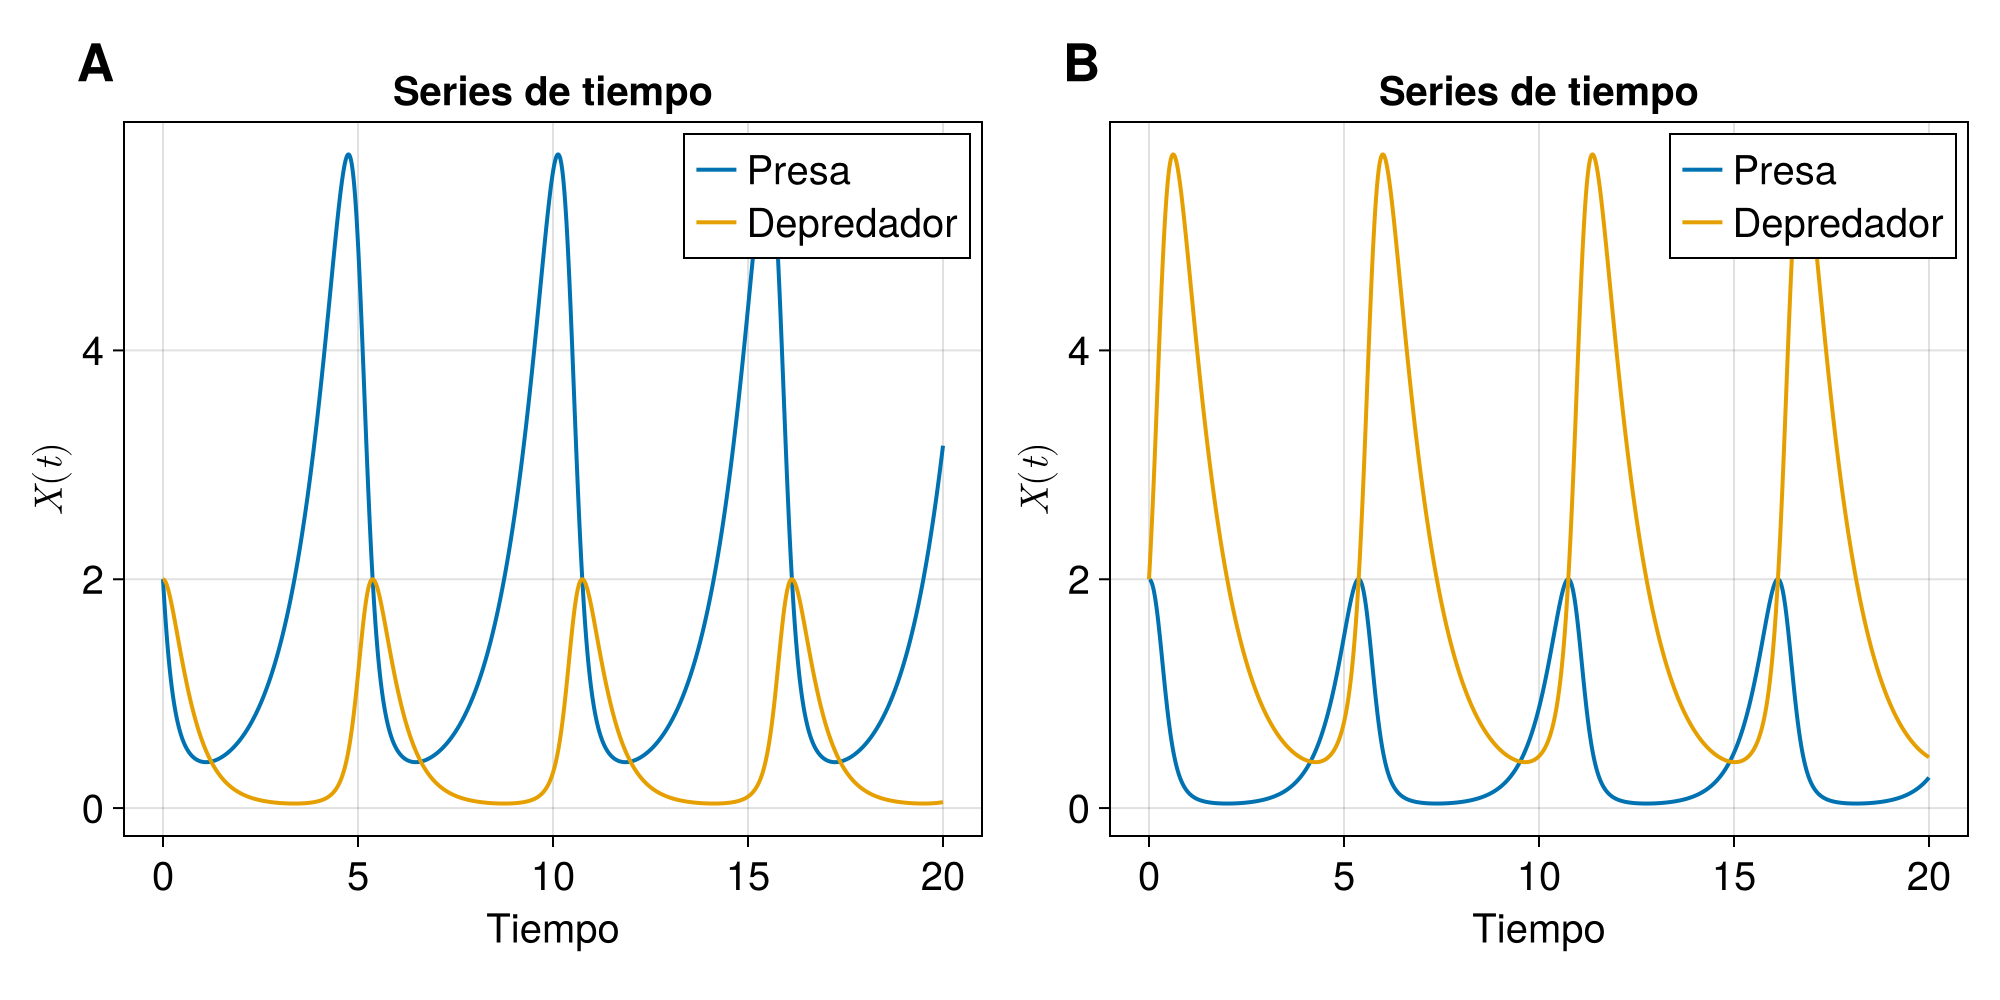
\includegraphics[scale=0.23]{../Imagenes/Series de Tiempo PD}
	\caption{(\textbf{A}) Serie de tiempo del sistema presa-depredador con $\alpha=1$, $\beta=2$, $\gamma=2$ y $\delta=1$. Bajo esta configuración la población de las presas se mantiene predominante sobre la población de depredadores. (\textbf{B}) Serie de tiempo del sistema presa-depredador con $\alpha=2$, $\beta = 1$, $\gamma = 1$ y $\delta = 2$. En este escenario la población de depredadores se mantiene predominante frente a la población de presas.}
	\label{fig:SeriesdeTiempoPD}
\end{figure}
En cambio para que los depredadores puedan predominar en su población solo hay que invertir las desigualdades propuestas y observar como con una alta natalidad de presas (abundancia) y un índice de depredación mayor a la mortalidad de los depredadores hace que se mantengan en mayor abundancia que las presas. En la Figura (\ref{fig:SeriesdeTiempoPD}) se aprecian ambos comportamientos antes descritos: Para la gráfica \textbf{A} se cumple el primer caso en donde $\alpha<\beta$ y $\delta<\gamma$ y se observa como las presas predominan en población frente a los depredadores mientras que en la gráfica \textbf{B} se cumple el segundo caso $\alpha>\beta$ y $\delta>\gamma$ confirmando que los depredadores predominan sobre las presas en su población. Aunque esto pueda ser un comportamiento general, se ha de aclarar que las formas de dinámica también dependerán de las condiciones iniciales, es decir que la predominancia de cada caso se cumplirá pero la forma de hacerlo irá cambiando\footnote{Es probable que existan más comportamientos en función de los coeficientes, sin embargo no se ahondará más en el tema y se invita al lector explorar más combinaciones que puedan surgir otro tipo de resultados.}.\\
\\
Para analizar más sobre la dinámica del sistema convendría conocer los puntos críticos del sistema y averiguar de que tipo de estabilidad se trata. El punto crítico trivial sabemos que es el $(0,0)$ y siempre será un repulsor, pues las poblaciones tienden a crecer ya sea en mayor o en menor medida. Igualando las ecuaciones de (\ref{eqn:PresaDepredador}) a cero y realizando las cuentas correspondientes se encuentra que el otro punto crítico es $(\frac{\gamma}{\delta},\frac{\alpha}{\beta})$. Por ahora no podemos determinar de manera analítica el tipo de estabilidad que producen puesto que no tenemos disponible una matriz de interacciones (originario de un sistema lineal) de la que podamos sacar eigenvalores para realizar el análisis de la sección anterior pero podemos guiarnos a partir de su espacio fase y ver que dinámica presenta.
\begin{ejemplo}\label{eg:PresaDepredador}
	Se define el siguiente sistema de presa-depredador para analizar el tipo de dinámica que produce
	\begin{equation}\label{eqn:EgPresaDepredador}
		\begin{split}
			\dot{x} &= 2x-0.6xy \\
			\dot{y} &= 0.5xy-2y
		\end{split}
	\end{equation}
	\begin{figure}[h!]
		\centering
		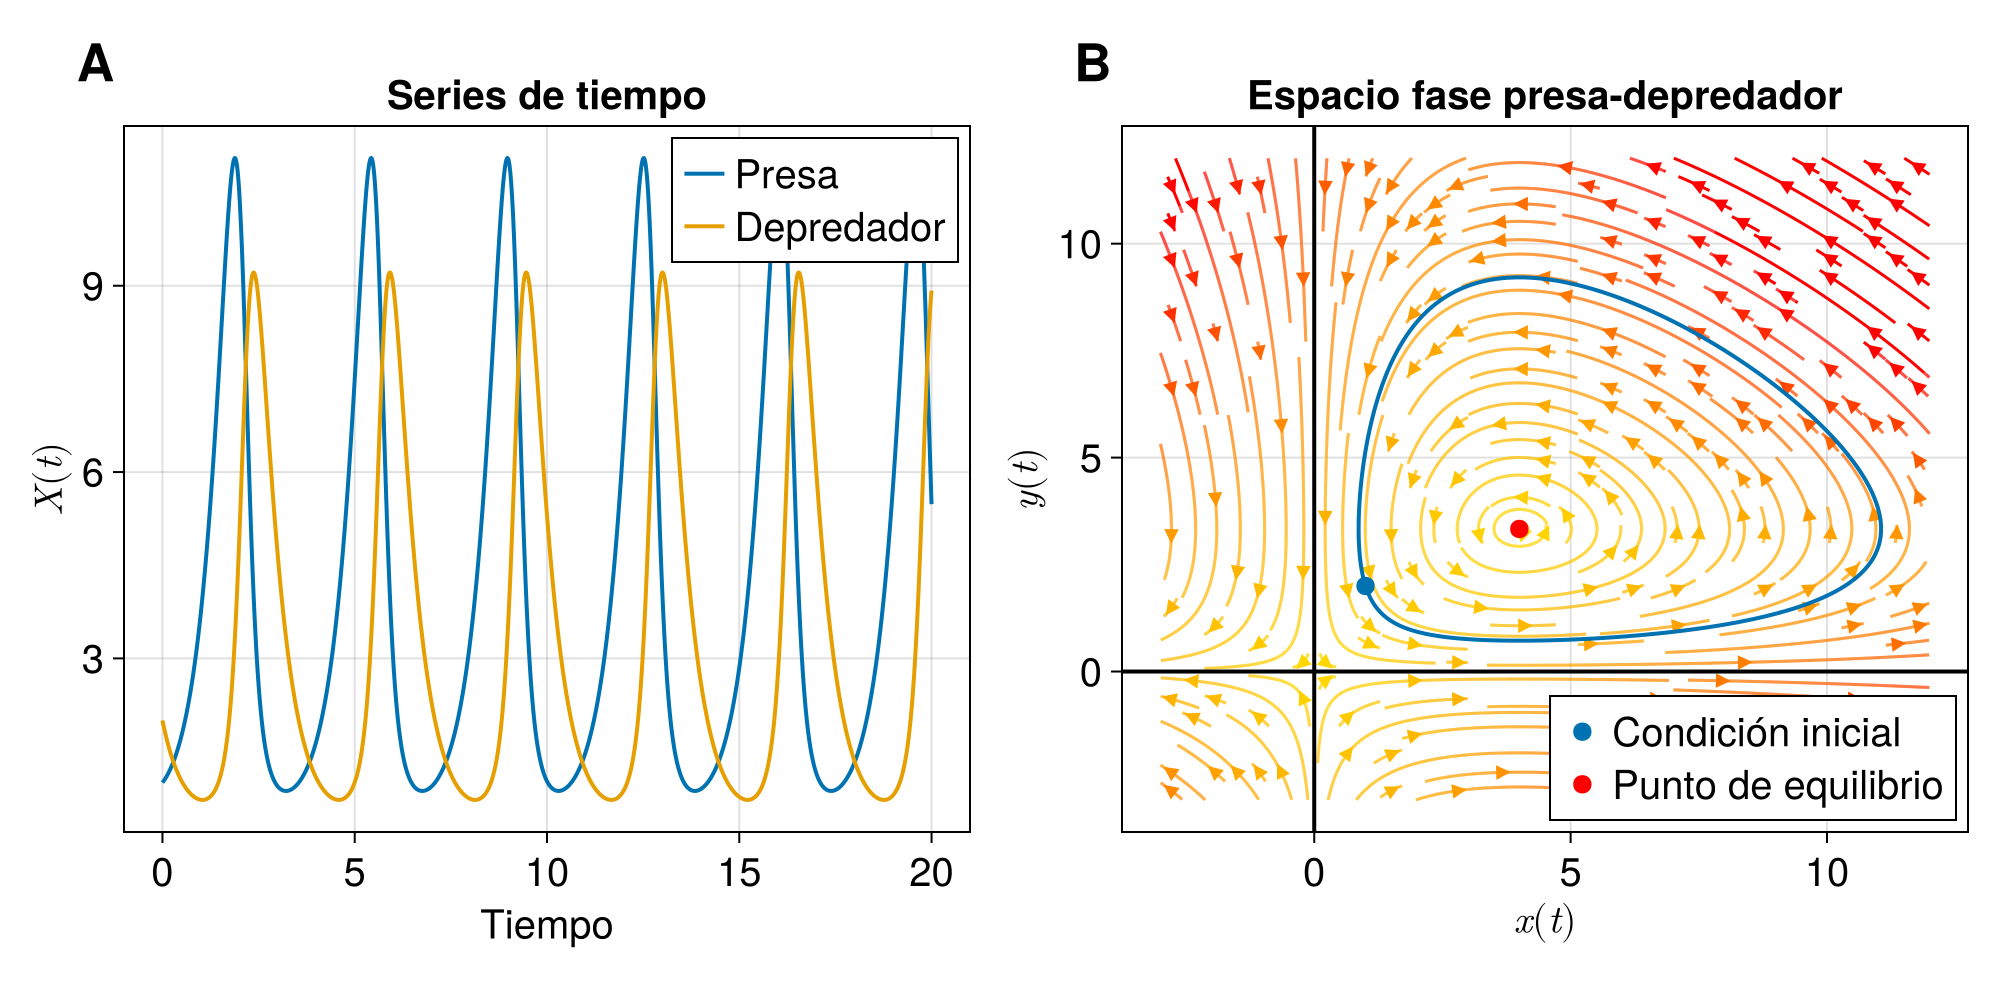
\includegraphics[scale=0.215]{../Imagenes/Espacio fase PD}
		\caption{(\textbf{A}) Serie de tiempo del sistema (\ref{eqn:EgPresaDepredador}) integrado con RK4 con un paso de integración $h=0.01$ y con la condición inicial $(1,2)$. (\textbf{B}) Espacio fase del sistema (\ref{eqn:EgPresaDepredador}) junto con la solución numérica marcada en azul.}
		\label{fig:EspacioFasePD}
	\end{figure}
	los puntos fijos del sistema son: $(0,0)$ y $(\frac{10}{3},4)$ respectivamente. En la discusión realizada anteriormente podemos anticipar que la población de presas predomina sobre la población de depredadores ya que $\alpha>\beta$ y $\gamma>\delta$ pero contamos con que $\beta>\delta$ y se propuso que la tasa $\beta$ ayuda al crecimiento de las presas por la alta demanda de depredación que en conjunto con el alto índice de mortalidad provoca que los depredadores tengan una etapa crítica de baja población. La Figura (\ref{fig:EspacioFasePD}) muestra la evolución temporal de las presas y los depredadores así como el espacio fase que cuenta con todas las soluciones posibles, en particular se marca en azul la que corresponde con el sistema (\ref{eqn:EgPresaDepredador}). La forma en que se obtuvo la solución fue por medio de integración numérica RK4 y constantemente se estará utilizando para la integración de los sistemas no lineales que se abordarán más adelante.\\
	\\
	En el espacio fase se puede notar como el $(0,0)$ es un punto fijo inestable ya que las soluciones pueden oscilar pero nunca convergen ni divergen absolutamente a dicho punto. Para el caso de $(\frac{\gamma}{\delta},\frac{\alpha}{\beta})$ se puede considerar como un centro ya que las soluciones tampoco convergen ni divergen solo oscilan, esto como muestra del comportamiento cíclico de este sistema.
	
\end{ejemplo}
\newpage
En el siguiente capítulo se abordará una técnica analítica para poder determinar la estabilidad de los puntos críticos de sistemas no lineales, se le conoce como \textit{Linealización} y aunque es una herramienta limitada que funciona a nivel local, sirve de mucho para explorar la estabilidad de sistemas no lineales de más de tres ecuaciones en donde la implementación visual es imposible de generar. Las aplicaciones de este modelo pueden variar desde su inmediato que es en ecología, en dinámica de enfermedades tal como lo es el modelo SIR, inclusive hasta en mercadología para ver que empresas dominan sobre otras o que acciones dominan sobre otras.
%%%%%%%%%CHECKPOINT
\subsubsection*{Introducción al modelo especies en competencia}

El sistema de presa-depredador se puede extender al realizar una combinación sutil con la ecuación logística (\ref{eqn:EqLogistica}), es decir, es agregarle una capacidad de carga y la premisa de que ahora no hay especies que depredan y que son depredadas sino que ahora las especies compiten por los recursos disponibles y finitos de un ambiente/ecosistema. Este es el conocido \textit{sistema de competencia de especies} o de Lotka-Volterra de competencia
\begin{equation}\label{eqn:CompentenciaEspecies2x2}
	\begin{split}
		\frac{dx}{dt} &= \alpha x\left (1-\frac{x}{k_1}\right )-\beta xy\\
		\frac{dy}{dt} &= \gamma y\left (1-\frac{y}{k_2}\right )-\delta xy
	\end{split}
\end{equation}
Este sistema de ecuaciones aumenta el número de términos no lineales con respecto del presa depredador, teniendo $x^2$ y $xy$ (para el caso de $\dot{x}$) por lo que también aumenta la complejidad al quererlo resolver de forma analítica\footnote{Si es que tiene solución.}. Aunque en el apéndice se presenten las soluciones analíticas de la ecuación logística y del sistema presa-depredador, para este sistema únicamente nos estaremos guiando de la solución numérica y los espacios fase que podamos generar computacionalmente para sistemas de 2 ecuaciones.\\
\\
El siguiente capítulo estará enteramente dedicado al sistema de especies en competencia, se abordarán desde lo particular con ejemplos de dos ecuaciones, se explorará su dinámica y se presentará la técnica de la linearización para poder determinar la estabilidad de los puntos fijos del sistema a nivel local. Posteriormente se generalizará el sistema a $N$ ecuaciones diferenciales y se hablará sobre las interacciones y su construcción. Se hablará sobre la implementación computacional para poder resolver el sistema generalizado de $N$ especies y se hablará sobre las condiciones para que el sistema pueda ser estable o no. El objetivo final de este trabajo es validar para que condiciones un sistema de $N$ ecuaciones diferenciales es estable y para cuales no lo es. Con base en ello se plantea la siguiente hipótesis
\newpage
\begin{proposición}
	Un sistema de competencia de especies generalizado de $N$ ecuaciones diferenciales presenta una transición de fase entre un régimen estable y otro inestable. Dicha transición esta determinada en función de los parámetros: $N$ número de especies (ecuaciones diferenciales), $p$ una probabilidad que determina la conectividad entre especies siendo que para valores de $p$ cercanos a cero el número de conexiones entre especies es bajo y para valores de $p$ cercanos a uno el número de conexiones entre especies es alto. Y por último $\sigma$ un parámetro que determina que tan ``fuertes" son las interacciones entre especies, es decir que tan altas o bajas son las tasas de interacción entre especies. 
\end{proposición}